% @TODO Change this
\chapter{Something "W" This Way Comes!}
\label{chapter4}

We will now continue our discussion on W-Structures in a more formal setting. In this chapter we will develop theory that captures their informal description we outlined previously. We will use it to construct three general algorithms for the detection of the largest w-structure in a height tree. We will describe the algorithms with pseudocode and provide the reader with proofs of correctness. Finally we will also demonstrate formal bounds on the time and space complexity of the proposed algorithms.

\section{Formal Description of W-Structures}


% @TODO Is this really a path definition?

We are interested in describing paths in height trees which form the characteristic zigzag pattern we described in Chapter 3. Let us first establish some of the basic notation we shall make use of. We will consider paths to be a sequence of distinct and adjacent vertices. When dealing with paths in height trees will often refer to them through their first and last vertex, because there is a unique path between any two vertices in a tree. For example when dealing with the path $v_1, v_2, v_3, v_4$ we will denote it with the shorthand $v_1 \rightsquigarrow v_4$. Lastly, a subpath of a path $P$ is a path whose vertices are also vertices of $P$. 

The first important property of paths in height trees we will define is their monotone path decomposition. The monotone path decompositino of a path $P$ as a sequence of vertexwise maximal monotone subpaths of $P$ where consecutive subpaths share exactly one vertex and have alternating direction.  As shown in Figure [] $P$ can be decomposed into the sequence of paths $P_1, P_2, ..., P_k$ such that $P_i \subseteq P$, $|P_i \cap P_{i+1}| = 1$ and $P_i \cup P_{i+1}$ is not a monotone path for $i \in \{1, 2, ..., k-1\}$ and $k \ge 1$. We can use the number of paths in the monotone path decomposition to characterise paths in height trees. To simplify this characterisation note that the number of subpaths in the monotone decomposition is exactly the number of vertices in which we change direction as we traverse the path. We shall name those special vertices kinks.

%The maximum path with respect to this property is precisely the lower bound on the parallel algorithm introduced in []. As a special case we must note that paths that can be decomposed into less than four monotone paths do not pose an algorithmic problem.


A kink in a path is a vertex whose two neighbours are either both higher or both lower (Figure []). Given the path $(u_1, u_2, ... , u_k)$ an inside vertex $u_i \ne u_1, u_k$ is a kink when $h(u_i) \notin \big( min(h(u_{i-1}),~h(u_{i+1}),~max(h(u_{i-1}),~h(u_{i+1}) \big)$. To avoid this cumbersome expression we shall adopt a slight abuse of notation and in the future write it as $h(u_i) \notin $ or $ \in $ $\big(h(u_{i-1}),~h(u_{i+1}) \big)$ where it will be understood that the lower bound of the interval is the smaller of the two and the upper bound the larger.


We can use the number of kinks in a path to define a metric on it. We will call this metric the w-length of a path and use it to measure the number of inside vertices of a path which are kinks. This is similar to how the length of a path is a metric that measures the number of edges between its vertices. The notation we will adopt for the w-length and length of a path $u \rightsquigarrow u$ is $w(u, v)$ and $d(u, v)$ respectively. There is not ambiguity here because as we have already said there is a unique path between any two vertices in a tree.  

In Chapter 3 we foreshadowed our intention of obtaining the largest W-Structure in a given contour tree. We can now put his in more precise terms as the path in a height tree that has the maximum w-length (or the longest w-path). We can immediately obtain a brute force approach for this problem by considering all paths in the height tree and computing their w-length to find the maximum one. This can be expressed with the following optimization term

$$ \max_{u, v \in V(T)}\{ w(u, v) \} .$$

The search space is quadratic in the number of vertices and measuring the w-length of a given path can be done by inspecting the height of every inside vertex and it's two neighbours in the path. The worst case running time of this algorithm is $O(d*n^2)$ where $d$ is the diameter (longest path) of the tree and $n$ is the number of vertices. This is however far from satisfactory given that the worst case time complexity of the algorithm for computing the contour tree is close to linear. We can in fact do better. 

The parallel we made between the w-length and length of a path has a deeper consequences. It we were to instead ask the question of finding the longest path in a tree we would find that it is a well studied problem. Our goal now will to try to transfer that knowledge to our task at hand. We will do so by analysing how two of the most popular algorithms for computing the longest path in a tree work and whether they can be adapted to instead find the longest w-path in a tree.  

%As the reader may have noticed the definitions we have made so far are analogous to the task of computing the longest path between any two vertices of a tree. This is completely intentional as we will demonstrate how algorithms for computing the longest path in a tree can be modified to produce the longest w-path instead. Finding the longest path of a graph in the general case is an \em NP-hard\em. Fortunately the Contour Tree is a tree. The longest path in a tree is known in the literature as it's diameter and has a polynomial time algorithm. The two most popular linear time algorithms found in the literature I will denote as Double Breadth First Search (2xBFS) and Dynamic Programming (DP). We will now take a look at how these algorithms work and hint at how they can be adapted in the next chapter.

\section{Tree Diameter Algorithms}

The longest path in a graph is an \em NP-hard \em problem. This can be demonstrate via a reduction to the Hamiltonian path problem []. Fortunately in the special case where the graph is a tree it has a linear time solution. In this special case it is known as the tree diameter problem. In this section we will take a look at how two of the linear time tree diameter problems work.


\subsection{Breadth First Search}

The first algorithm we will discuss is based on the following theoretical result [].

\begin{lem} Let $s$ be any vertex in a tree. Then the most distant vertex from $s$ is an endpoint of a tree diameter. \end{lem}

    To implement this algorithm we require of way of finding the most distant vertex from a given vertex. This can be done using Breadth First Search (BFS). Let $T$ be a tree and $s \in V(T)$ be any vertex. We can run BFS with $s$ as its root to find a vertex $u$ such that $d(s, u) \ge d(s, t)$ for all $t \in V(T)$. We can then run a second BFS with root $u$ to obtain a vertex $v$ such that $d(u, v) \ge d(u, t)$ for all $t \in V(T)$. As $u$ is the farthest vertex from $s$ it must be the endpoint of a diameter. As the diameter of $T$ is the longest path in $T$ therefore the second BSF must produce a path of length as much as the diameter. Therefore $d(u, v) \ge d(a, b)$ for all $a,b \in V(T)$. 

The space and time complexity of BSF are linear [] and therefore the space and time complexity of this algorithm are linear as well. This follows from that fact that the algorithm consists of running BFS just two consecutive times.

\subsection{Dynamic Programming}

The second approach is based on the Dynamic Programming paradigm. Dynamic Programming is a method that is used to solve optimisation problems that exhibit recursive substructures of the same type as the original problem. The key ingredients in developing a dynamic-programming algorithm are [Into to Algorithms]:


\begin{enumerate}
    \item Characterise the structure of the optimal solution.
    \item Recursively define the value of an optimal solution.
    \item Compute the value of the optimal solution.
\end{enumerate}

% @TODO Redefine N(u)

Trees exhibit optimal substructure through their subtrees. For our intents and purposes we shall define a subtree as a connected subgraph of a tree. We will only consider rooted trees in the context of this algorithm and we must define the accordingly. Let $T$ be a rooted tree and let $v, u \in V(T)$ be two vertices such that $v$ is the parent of $u$. We shall define the subtree rooted at $u$ as the maximal (vertex-wise) subgraph of $T$ that contains $u$ but does not contain $v$.  We will denote it as $T_u$. In this notation $T = T_s$ where $s$ is the root of $T$. The rooted subtree at $u$ is smaller than $T$ as it does not contain at least one of the vertices of the $T$ namely - $v$. The structure of the optimal solution is characterised through all possible rooted subtrees $\{T_u\}_{u \in V(G)}$.

We can recursively define the value of the optimal solution with the following observation. Starting at the root of the tree the longest path in tree either goes through two children of the root and the root or is entirely contained in one of the subtrees rooted at one the children. In order to define this formally we will make use of two additional functions. Let $h(u)$ be the height of the subtree rooted at $u$. The height is defined as the longest path in $T_u$ from $u$ to one of the leaves of $T_u$. We will also define $D(u)$ as longest path contained entirely in $T_u$. The function we will maximize is $D(s)$ where $s$ is the root of $T$. We will do so with the following formula.

$$ D(v) = max\bigg\{ \max\limits_{u \in N(v)}\bigg(D(u)\bigg), \max\limits_{u, w \in N(v)}\bigg(h(u) + h(w) + 2\bigg) \bigg\}. $$

The base case for this recursive formula is at the leaves of $T$. If $u$ is a leaf of $T$ then $V(T_u) = \{u\}$. This allows us to set $h(u) = 0$ and $D(u) = 0$ and consider all leaves as base cases for the recursive formula. We are guaranteed to reach the base case as each subtree is strictly smaller we must inevitably reach all leaves.

This algorithm can be implemented in linear time using Depth First Search (DFS) by using two auxiliary arrays that hold the values for $h(u)$ and $D(u)$ for every $u \in V(T)$. We will omit going into more details at this point and refer the reader to [] for the implementational details and proof of correctness and running time. 

%@TODO Fix sentece before

\section{Tree W-Diameter Algorithms}

We will now step into the realm of w-detection. Before we outline the proposed algorithms we must establish two key properties which hold the difference between the tree diameter algorithms and their modification to tree w-diameter algorithms.

\begin{defn} Subpath Property  \end{defn}

Let $a \rightsquigarrow b$ be a path and $c \rightsquigarrow d$ it's subpath. Then $w(a, b) \le w(c, d)$. 

This property follows from the fact that all kinks of the path from $c$ to $d$ are also kinks of the path from $a$ to $b$. An important thing to note is that in the case of path length if one of the paths is a proper subpath of the other then the inequality is strict. This does not have to be the case with w-paths for the w-length, decreases only when we remove a kink from a path.

\begin{defn} Path Decomposition Property Property  \end{defn}

    Let $a \rightsquigarrow b$ be the path $(a, u_1, u_2, ..., u_k, b)$ and $u_i$ be an inside vertex for any $i \in \{1, 2, ..., k\}$. Then: 
    
    $$w(a, b) = w(a, u_i) + w(u_i, b) + w_{a \rightsquigarrow b}(u)$$
    
   where:
    
   $$
   w_{a \rightsquigarrow b}(u_i) = \left\{
       \begin{array}{@{}l@{\thinspace}l}
           \text{0}  &: \text{if } h(u_i) \in \big(h(u_{i-1}),~h(u_{i+1}) \big) \text{ // $u_i$ is not a kink} \\
           \text{1} &: \text{otherwise // $u_i$ is a kink.} \\
       \end{array}
   \right.
   $$

   Indeed $u_i$ can be a kink in the path from $a$ to $b$, but it cannot be a kink in the paths from $a$ to $u_i$ and from $u_i$ to $b$ because it is an endpoint of both. All other kinks are counted by either $w(a, u_i)$ or $w(u_i, b)$. When making use of path decomposition property in future proofs we must account for whether the vertex we are decomposing a path at is a kink in that path or not.


\subsection{Linear Time Algorithm - 2xBFS}

We shall first explore how we can modify the Double Breadth First Search algorithm to compute the w-diameter of a height tree. The new algorithm will follow exactly the same steps. The only exception is that it will run a modified version of BFS that computes w-distances [see algorithm next page] from a given root vertex to all others in the tree. The algorithm works by first running a BFS from any vertex in the graph and then records the leaf that is farthest in terms of w-length. This furthest leaf is guaranteed to be either the endpoint of a path in the tree whose w-length least that of the actual w-diameter of the tree minus two. 


\begin{algorithm}
\caption{Computing the W Diameter of a Height Tree.}

\begin{algorithmic}[1]

\Function{W\_BFS}{T, root}
    \State root.d = 0
    \State root.$\pi$ = root
    \State furthest = root

    \State Q = $\emptyset$
    \State Enqueue(Q, root)

    \While {Q $\ne \emptyset$}
        \State u = Dequeue(Q)

        \If {u.d $>$ furthest.d}
            \State furthest = u
        \EndIf

        \ForAll {v $\in$ T.$Adj$[u]} 
            \If {v.$\pi$ == $\emptyset$}
                \State v.$\pi$ = u
                \If {h(u) $\notin$ \big(h(v),~h(u.$\pi$)\big)}
                    \State v.d = u.d + 1
                \Else
                    \State v.d = u.d
                \EndIf

                \State Enqueue(Q, v)

            \EndIf
        \EndFor
    \EndWhile
    \State Return furthest
\EndFunction

\Function{Calculate\_W\_Diameter}{T}
    \State s = <any vertex>
    \State u = W\_BFS(T, s)
    \State v = W\_BFS(T, u)
    \State return v.d
\EndFunction

\end{algorithmic}
\end{algorithm}

%\newtheorem{w-algorithm}{The W Detection Algorithm is Correct.}
Before proving the correctness of the algorithm we must first establish two useful properties that relate the w-length of a path to it's subpaths.


\begin{lem} The Algorithm produces the endpoints of a path who is at most 2 kinks shy of being the kinkiest path in the tree. \end{lem}


\begin{proof}
Let $T$ be a height tree and $s \in V(T)$ be the initial vertex we start the first search at. After running the modified BFS twice we obtain two vertices $u$ and $v$ such that:

\begin{equation}
    \label{eq:su_all}
    w(s, u) \ge w(s, t), \forall t \in V(T)
\end{equation}

\begin{equation}
    \label{eq:uv_all}
    w(u, v) \ge w(u, t), \forall t \in V(T)
\end{equation}

Furthermore let $a$ and $b$ be two leaves that are the endpoints of a path that is a w-diameter. For any such pair we know that:

\begin{equation}
    \label{eq:ab_all}
    w(a, b) \ge w(c, d), \forall c, d \in V(T)
\end{equation}

By this equation we have that $w(a, b) \ge w(u, v)$. Our goal in this proof will be to give a formal lower bound on $w(u, v)$ in terms of $w(a, b)$. To this end let $t$ be the first vertex in the path between $a$ and $b$ that the first BFS starting at $s$ discovers. We can infer that $t$ cannot be $a$ or $b$ unless $s$ is equal to $a$ or $b$.

The proof can then be split into several cases depending on the relative positions of $s$, $t$, $a$, $b$ and $u$. \linebreak

{\em Case 1. When the path from $a$ to $b$ does not share any vertices with the path from $s$ to $u$.}

{\em Case 1.1. When the path from $u$ to $t$ goes through $s$.}



% @TODO Explain that the dotted lines are paths.
\begin{figure}%
    \centering
    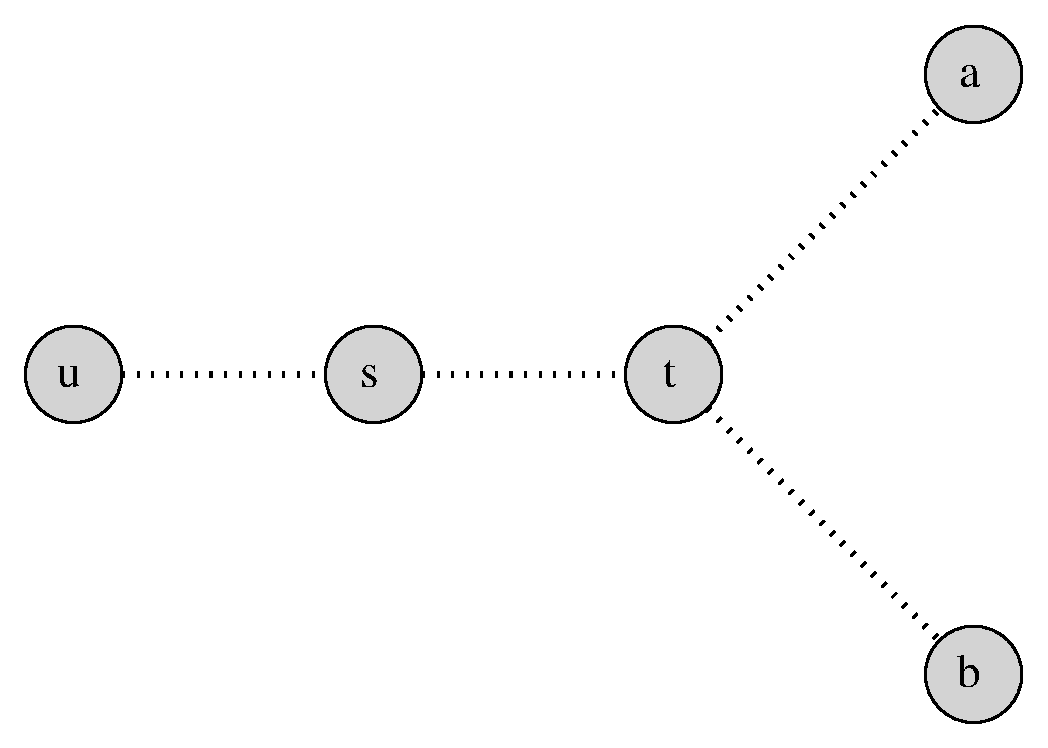
\includegraphics[center, scale=0.5 ]{./images/2xbfs-case-1-1.eps}
    \caption{Relative position of vertices in Case 1.1 }%
    \label{fig:case1.1}%
\end{figure}

In this case $s \rightsquigarrow u$ is a subpath of $t \rightsquigarrow u$, which in turn means that $w(t, u) \ge w(s, u)$. By equation \ref{eq:uv_all} we also have that $w(s, u) \ge w(s, a)$. We can therefore conclude that $w(t, u) \ge w(a, t)$ as $s \rightsquigarrow a$ is a subpath of $t \rightsquigarrow a$.

Now via path decomposition of $a \rightsquigarrow b$ and $u \rightsquigarrow b$ at $t$ have that:

$$ w(a, b) = w(b, t) + w(t, a) + x  $$
$$ w(u, b) = w(b, t) + w(t, u) + y .$$

Where $x, y \in \{0, 1\}$ depending on whether there is a kink at $t$ for the path from $a$ to $b$ and from $u$ to $b$ respectively. As $w(t, u) \ge w(a, t)$ we can show that:


$$ w(u, b) \ge w(b, t) + w(t, a) + y $$
$$ w(u, b) \ge w(b, t) + w(t, a) + x - x + y $$
$$ w(u, b) \ge w(a, b) - x + y $$
$$ w(u, b) \ge w(a, b) + (y - x) $$

But as $w(u, v) \ge w(u, b)$ (by equation \ref{eq:uv_all}) we obtain that: Sha
$$ w(u, v) \ge w(a, b) + (y - x) $$

Considering all possible values that $x$ and $y$ can take, we can see that the minimum value for the right hand side of the inequality is at $y = 0$ and $x = 1$. The final conclusion we may draw is that $w(u, v) \ge w(a, b) -1$.



%$a\rightsquigarrow b$

{\em Case 1.2. When the path from $u$ to $t$ does not go through $s$.}

\begin{figure}%
    \centering
    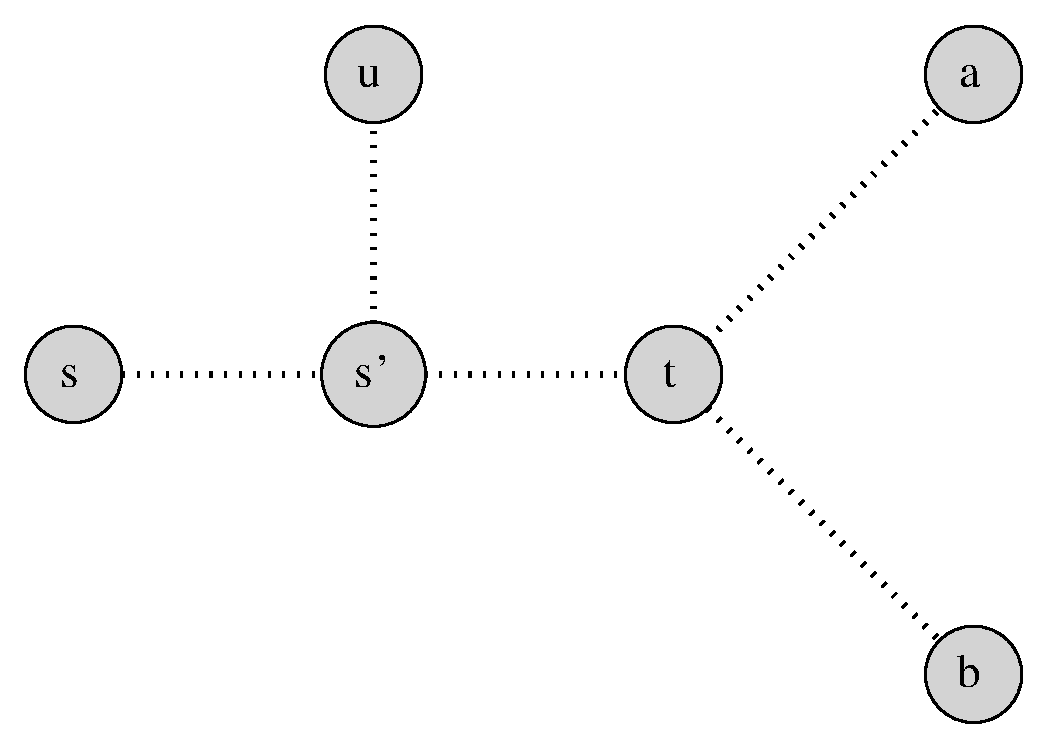
\includegraphics[center, scale=0.5 ]{./images/2xbfs-case-1-2.eps}
    \caption{Relative position of vertices in Case 1.2 }%
    \label{fig:case1.2}%
\end{figure}

If the path from $u$ to $t$ does not go through $s$ then the paths $s \rightsquigarrow t$ and $s \rightsquigarrow u$ have a common subpath. Let $s'$ be the last common vertex in that subpath. We will be able to produce s proof that is similar to the previous case by considering $s'$ in the place of $s$. We must only account for whether $s'$ is a kink in one of the paths $s \rightsquigarrow u$ or $s \rightsquigarrow t$. We know that $w(t, u) \ge w(s', u)$ (as a subpath) and through path decomposition of  $s \rightsquigarrow a$ and $s \rightsquigarrow u$ at $s'$ we obtain that:

$$ w(s, a) = w(s, s') + w(s', a) + x $$
$$ w(s, u) = w(s, s') + w(s', u) + y $$

where $x,y \in \{0, 1\}$ indicate whether $s'$ is a kink in the corresponding path as before. By equation \ref{eq:su_all} we know that $w(s, u) \ge w(s, a)$ and therefore:

$$ w(s, s') + w(s', u) + y \ge w(s, s') + w(s', a) + x  $$ 
$$ w(s', u) + y \ge w(s', a) + x $$ 
$$ w(s', u) \ge w(s', a) + (x - y).$$ 

Since $s'$ lies on the path from $t$ to $u$ we have that $w(t, u) \ge w(s', u)$ by the subpath property. We can use this to conclude the following:

$$ w(t, u) \ge w(s', a) + (x - y).$$ 

From the fact that $t \rightsquigarrow a$ is a subpath of $s' \rightsquigarrow a$ it follows that $w(s', a) \ge w(t, a)$. This allows us to infer that:

$$ w(t, u) \ge w(t, a) + (x - y). $$ 

Now we are ready to proceed in a similar manner as the previous case. We will decompose the paths from $b$ to $a$ and from $b$ to $u$ at the vertex $t$ as follows:

$$ w(b, a) = w(b, t) + w(t, a) + z  $$
$$ w(b, u) = w(b, t) + w(t, u) + w  $$
$$ w(b, u) \ge w(b, t) + w(t, a) + (x - y) + w $$
$$ w(b, u) \ge w(b, t) + w(t, a) + z - z + (x - y) + w $$
$$ w(b, u) \ge w(a, b) - z + (x - y) + w $$
$$ w(b, u) \ge w(a, b) + (x - y) + (w - z) $$

The minimum value for the right hand side of this equation is at $x, w = 0$ and $y, z = 1$. Using the fact that $w(u, v) \ge w(u, b)$ we finally obtain $ w(u, v) \ge w(a, b) - 2 $.


{\em Case 2. When the path from $a$ to $b$ shares at least one vertex with the path from $s$ to $u$.}

\begin{figure}%
    \centering
    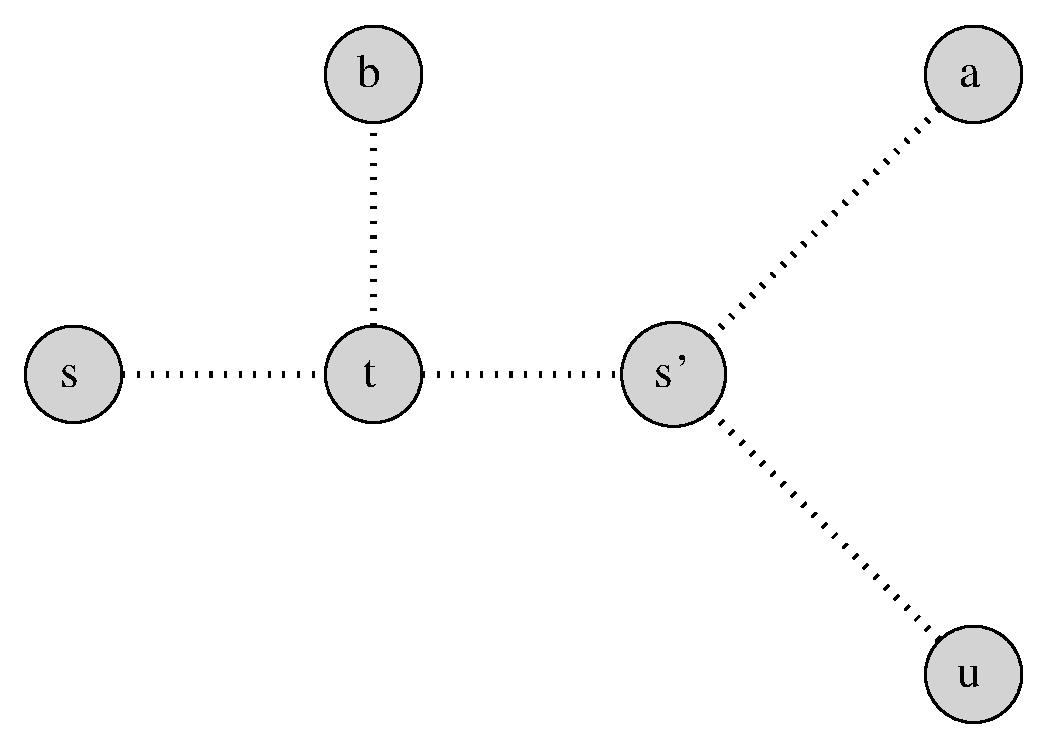
\includegraphics[center, scale=0.5 ]{./images/2xbfs-case-2.eps}
    \caption{Relative position of vertices in Case 2 ($t$ could be equal to $s'$). }%
    \label{fig:case2}%
\end{figure}

% @TODO This is not complete!
%As we already know $w(s, u) \ge w(s, a)$. Furthermore $w(s, u) \ge w(t, u)$ and $w(s, a) \ge w(t, a)$ as they are subpaths of $s \rightsquigarrow u$ and $s \rightsquigarrow a$ respectively. Therefore $w(t, u) \ge w(t, a)$. We can now decompose the paths from $b$ to $a$ and from $b$ to $u$ at the vertex $t$ as follows:

We can do a path decomposition as follows:

$$ w(s, u) = w(s, t) + w(t, u) + x $$
$$ w(s, a) = w(s, t) + w(t, a) + y $$

As $w(s, u) \ge w(s, a)$ (by equation \ref{eq:uv_all})we obtain that:

$$ w(s, t) + w(t, u) + x  \ge w(s, t) + w(t, a) + y $$
$$ w(t, u) \ge w(t, a) + (y - x) $$

If we again decompose the paths from $b$ to $a$ and from $b$ to $u$ at $t$ we obtain:

$$ w(b, a) = w(b, t) + w(t, a) + z  $$
$$ w(b, u) = w(b, t) + w(t, u) + w  $$
$$ w(b, u) \ge w(b, t) + w(t, a) + (x - y) + w $$
$$ w(b, u) \ge (w(b, t) + w(t, a) + z) - z + (x - y) + w $$
$$ w(b, u) \ge w(a, b) - z (x - y) + w $$
$$ w(b, u) \ge w(a, b) + (x - y) + (w - z). $$

Where similarly to the previous case the rightful conclusion is that $ w(u, v) \ge w(a, b) - 2 $.

Based on these cases we can have shown that that for any input tree the algorithm will produce a w-path that is at most two kinks less than the actual maximum w-path.


\end{proof}

\begin{lem} The time complexity of the algorithm is $O(|V|)$. \end{lem}

\begin{proof}
    The modified BFS function has the same time complexity of BFS as all we have added is an "\em if, then, else\em"~statement. The time complexity of BFS is $O(|V| + |E|)$, but in a tree $|E| = |V| - 1$, so the overall complexity is $O(2|V| - 1) = O(|V|)$. 
    Running the modified BFS function twice remains in linear, thus the overall complexity of the algorithm is linear as well.
\end{proof}

\begin{lem} The space complexity of the algorithm is $O(|V|)$. \end{lem}

\begin{proof}
    Completely analogous to the standard BFS algorithm, this algorithm uses the same amount of memory in the standard memory model.
\end{proof}

\subsection{Pathological Cases in 2xBFS}

Here are examples of the pathological case where the w-diameter outputted by the 2xBFS algorithm is different than the actual w-diameter. Look at Fig. \ref{fig:path-cases}. There is one example corresponding to all proof cases. In all the examples the vertex outputted by the first BFS function would be $u$ after which the longest path would be outputted as $u \rightsquigarrow a$ or $u \rightsquigarrow b$. The problem is that $w(u, a) = w(u, b) = 1$, but $w(a, b) = 1$ or $2$ in the first example. Note that even if we adapt the algorithm so that it finds the vertex with largest w-length away and breaks ties with normal distance, we will still be able to apply these examples. We just need to augment them by subdividing the path to $u$ to make if further away from $a$ and $b$, but keep the same w-lenght between $s, a, b u$.

\begin{figure}%
    \centering

    \subfloat[Pathological Example for Case 1. 1 (-1 of actual w-diameter).]{{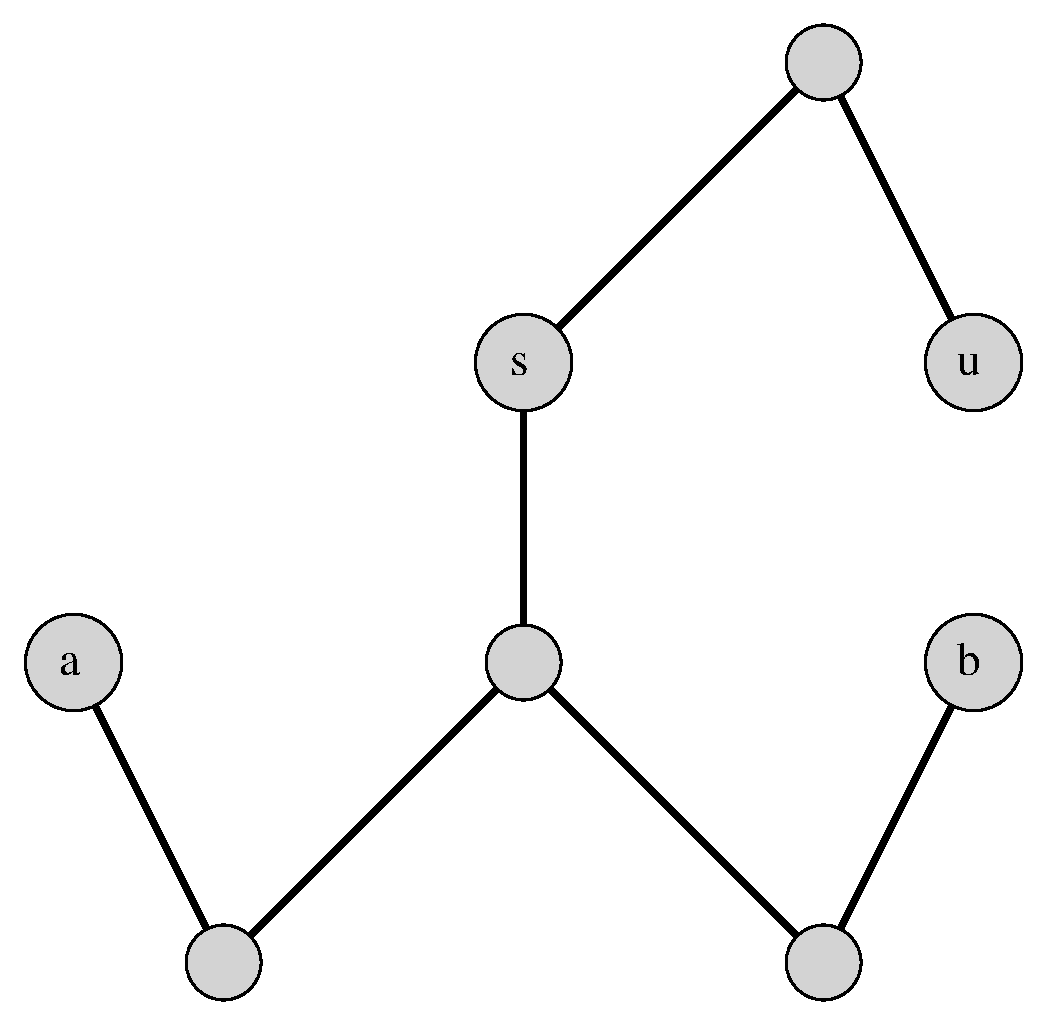
\includegraphics[scale=0.4]{./images/2xbfs-path-case-1-1.eps}}}%
    \qquad
    \subfloat[Pathological Example for Case 1. 2 (-2 of actual w-diameter).]{{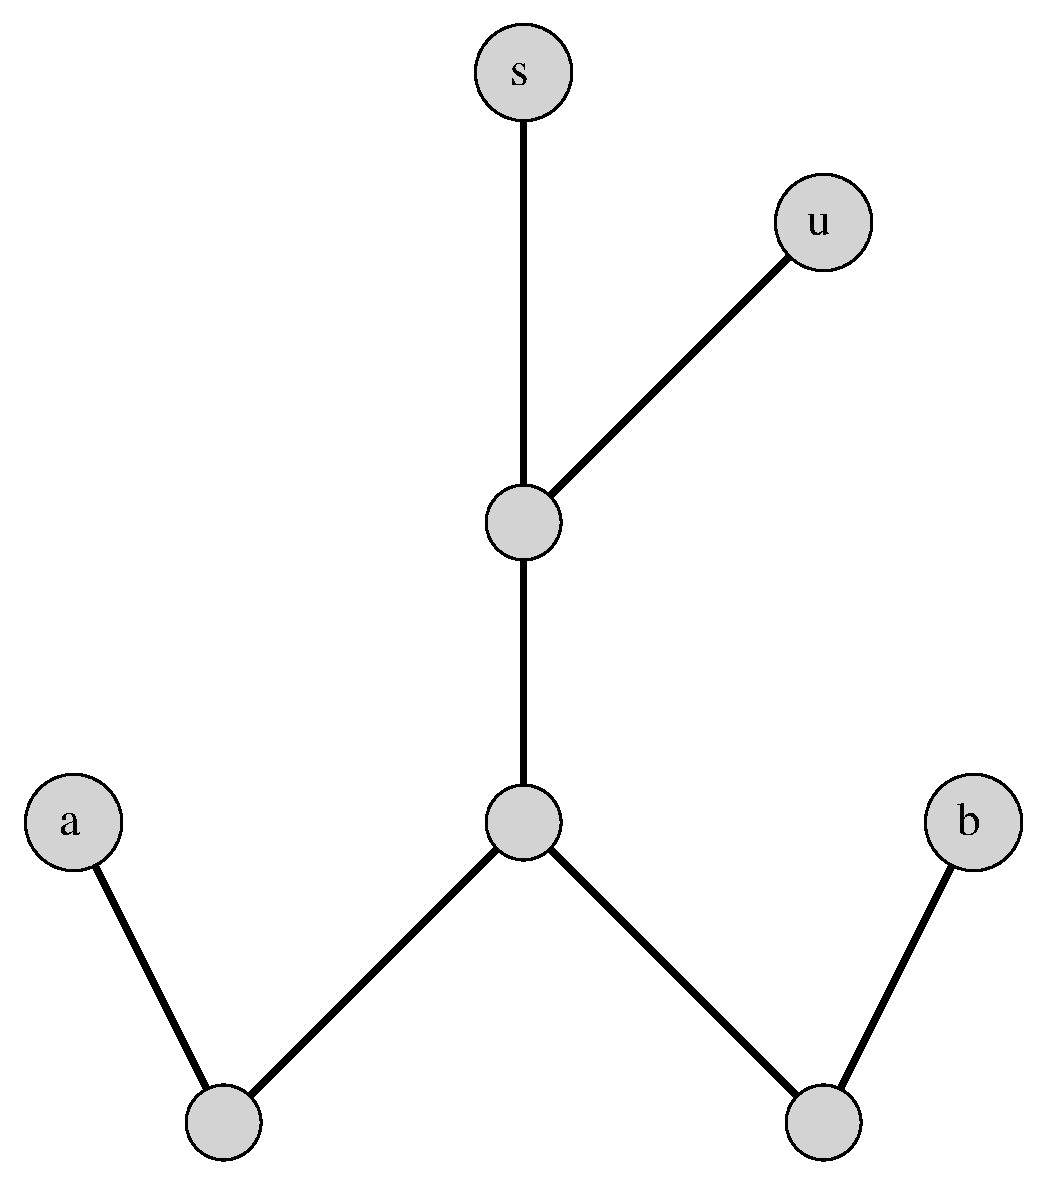
\includegraphics[scale=0.4 ]{./images/2xbfs-path-case-1-2.eps}}}%
    \qquad
    \subfloat[Pathological Example for Case 2 (-2 of actual 2-diameter).]{{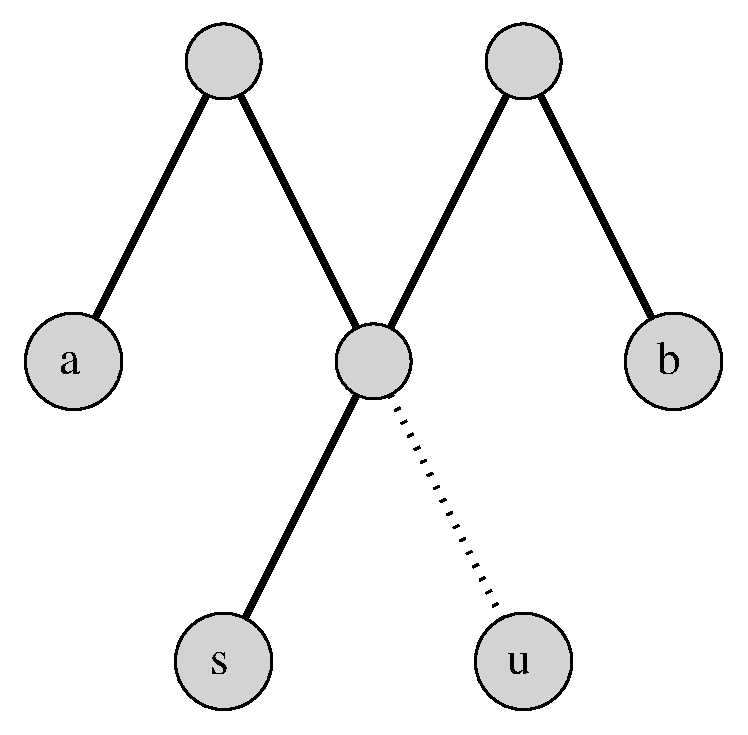
\includegraphics[scale=0.6 ]{./images/2xbfs-path-case-2.eps}}}%
    \caption{Branch Decomposition of a Contour tree.}%
    \label{fig:path-cases}%
\end{figure}



\subsection{Attempts at resolving the accuracy of 2xBFS}


% @TODO Chapter 3 here may change.

For the intents of purpose of this dissertation the accuracy of this algorithm is sufficient. In large enough data sets this estimate provides enough insight to correlate the observed iterations needed to collapse the split and join trees and the resulting w-diameter of the tree. This is demonstrated empirically in Chapter 3. Regardless of such practical considerations it is still of inherent theoretical interest to investigate how we may be able to obtain a more accurate modification of this algorithm.

One key observation we can make is that on the second run of the BFS we get a w-path that is necessarily longer or equal to one found in the first BFS search. A natural question to ask is whether running the BFS a third, fourth or for that matter nth time would result in the actual w-diameter. On every successive iteration we get a w-path that is longer or equal to the previous one, because w-length is a symmetric path property ($w(a, b) = w(b, a)$). By doing this we can hope that we will eventually obtain a w-path closer to the w-diameter. However there is no guarantee that this will happen. In fact in some cases it is possible that each successive BFS will return the same path over and over again. Obverse how in @TODO fig[] all iterations of BFS go from the vertex $u$ to the vertex $v$ and then from $v$ to $u$ and so on. 


A different heuristic we can apply is to run the algorithm multiple times from different starting points and keep the maximum value found. This approach is somewhat reliable, but may still fail to find the w-diameter. Consider @TODO fig[]. That artificial example shows that there can simply be too few starting points which would produce the w-diameter.


% @TODO Redo Last Paragraph.
In the search for a better solution let $s$ be a starting vertex and let the vertices $U = \{u_1, u_2, ..., u_n\}$ be the furthest away in terms of w-distance and $W = \{w_1, w_2, ..., w_n\}$ be the ones second furthest away. By the proof of the algorithm we know that not necessarily all vertices in those sets would produce a w-diameter. Thus lets us define $R \subseteq U \cup W$ as the set of vertices which are endpoints of a w-diameter. As we have shown we can construct an example where $|R| = 2$ and $|U \cup W|$ is arbitrarily large. Can we then find some property of the vertices in $R$ and pick them out in the first phase of the algorithm? *This I will leave open for the future generations to ponder. I hope in doing so all people of the world will unite unite and end all wars and prejudices in order to work towards this common good!*

\subsection{Dynamic Programming Algorithm - DP}


% @TODO 
*Idea redefine $N(u) = N(u) / u.\pi$ so you can simplify notation.*

While it is encouraging that we have obtained an algorithm that bounds the w-diameter it is also quite unsatisfactory that we were not able to directly obtain it. To remedy this we will resort to modifying the second tree diameter algorithm that we outlined previously. We will use the same optimisation strategy i.e. dynamic programming by making two key changes. Instead of the function $h(u)$ that computes the height of a subtree with root $u$ we will use the function $w(u)$ that stores the longest w-path that starts at the root of the subtree. We will remane the function that stores the value of the optimal solution for subroblems from $D(u)$ to $W(u)$ accordingly. To summarise $W(u)$ returns the length of the largest w-path in the subtree $T_u$ and $w(u)$ the length of the largest w-path in $T_u$ that starts at $u$.

This may seem like a simple substitution at first glance, but the devil is in the details. As in the previous modification all additional difficulties stem from the difference in combining path lengths and path w-lengths. Let us begin by examining how the w-height of a vertex is computed from the w-heights of its children. Let $s$ be a vertex in $T$ and let us assume the we have computed the w-heights of its children recursively. In the case of computing the height we can simply set $h(s) = \max\limits_{u \in N(s)}\big( h(u) \big) + 1$. We cannot do so with the w-height because w-length can remain the same if we do not extend the maximum w-path with a kink.  To demonstrate this let us assume that $u \in N(s)$ is such that $w(u) = \max\limits_{v \in N(s)}(w(v))$. Then if we wish to extend the maximum w-path that ends at $u$ to $s$ we must account for whether $u$ becomes a kink in it. If none of the children of $s$ with maximum w-height form a kink when extending to $s$ then the w-height of $s$ does not increase.

To see how we can obtain the w-height of $s$ let $u$ be any of it's children and $L_u = \{u_1, u_2, ..., u_k\}$ be all children of $u$ through which a w-path with length $w(u)$ passes through. Then we can compute the w-height of $s$ as: $w(s) = \max\limits_{u \in N(s)}\{ h(u) + \max\limits_{v \in L_u}(w_{s, v}(u)) \}$. In other words there may be multiple w-paths with the same maximal w-length that end at $u$. If possible we must pick the one that would make $u$ form a kink with $s$. If not we can use any of them. There is no point in looking at paths of lesser w-length as it can only increase by one and at best match the maximum ones.


In the tree diameter scenario path combination is straightforward. For a tree with root $s$ we first find two distinct children $u, v \in N(s)$ of $s$ such that $h(u)$ and $h(v)$ is maximum amongst all children and $u \ne v$ (otherwise we get a walk and not a path). Next we will combine them to obtain the longest path that goes through $s$. This path combination yield the sum $h(u) + h(v) + 2$, where we account for the two additional edges $us, sv \in E(T_s)$. This reasoning of course extends to all subtrees in $T$. In the latter case of w-path combinations we must be vigilant of which vertices become kinks in the path combinations. Let us observe a similar scenario where $s$ is the root the tree and $u, v \in V(T_s)$ are two of the children with maximal values for $w(u)$ and $w(v)$. We would ideally like to combine $w(u)$ and $w(v)$ like so: $w(u) + w(v) + w_{u, v}(s)$. This however is not correct! There is a hidden assumption in the sum that the only vertex that can become a kink in this path combination is $s$. Contrary to this, in fact $u$ and $v$ can also become kinks. Observe that $w(u) \text{ and } w(v)$ are the w-length of two paths - one starting at $u$ and ending in a leaf of $T_u$ and one starting at $v$ and ending in a leaf of $T_v$. In the new path, both $u$ and $v$ can become inside vertices and depending on whether they become kinks or not the sum may further increase by two. To account for this we must also look at the children of $u$ and $v$ through which a maximum w-path passes. 


This process is similar to the one for obtaining the w-height of a vertex and is described by the following formula: 

$$\max\limits_{\substack{u, v \in N(s) \\ u \ne v}}\{ h(u) + \max\limits_{t \in L_u}(w_{s, t}(u)) + h(v) + \max\limits_{t \in L_v}(w_{s, t}(v)) + w_{u, v}(s)\}$$

Thus the formula that describes the optimal solution can be written as:


% @TODO Finish This.

$$ W(s) = max\Bigg\{ \max\limits_{u \in N(s)}\bigg(W(u)\bigg), \max\limits_{\substack{u, v \in N(s) \\ u \ne v}} \bigg( h(u) + \max\limits_{t \in L_u}(w_{s, t}(u)) + h(v) + \max\limits_{t \in L_v}(w_{s, t}(v)) + w_{u, v}(s)\bigg) \Bigg\}. $$

As before the optimal solution is either entirely in one of the subtrees of the children of a vertex or in the path combination of two of the children of the vertex.

Here is the pseudocode for the algorithm.

\begin{algorithm}{}
\caption{Computing the W Diameter of a Height Tree.}
\begin{algorithmic}[1]

%\Function{W\_DFS}{T, s}
    \State{\textbf{Function}W\_DFS}(T, s)

    % If we are at a leaf Base Case
    \State // Base Case
    \If {|T.$Adj$[s]| == 1 AND s.$\pi \ne $ s}
        \State s.W = 0
        \State s.w = 0
        \State return
    \EndIf

    % Forwards DFS visit

    \State // DFS Visit
    \ForAll {u $\in$ T.$Adj$[s]} 
        \If {u.$\pi$ == $\emptyset$}
            \State u.$\pi$ = s
            \State W\_DFS(T, u)
        \EndIf
    \EndFor

    % Backtracking
    \\

    \State // After all neighbours are visited

    \State // Calculate w-height of s
    \ForAll {u $\in$ T.$Adj$[s]$/s.\pi$} 
        \If {L[u] == $\emptyset$}
            \State H[s] = max(H[s], H[u]);
        \Else
            \ForAll {v $\in$ L[u]$/u$} 
                \State H[s] = max(H[s], H[u] + $w_{v, s}(u)$);
            \EndFor
        \EndIf
    \EndFor

    \State // Find all children that contribute to the a w-height path
    \ForAll {u $\in$ T.$Adj$[s]$/s.\pi$} 
        \If {L[u] == $\emptyset$ AND H[s] == H[u]}
            \State L[s] = L[s] $\cup$ u
        \Else
            \ForAll {v $\in$ L[u]$/u$} 
                \If {H[s] = max(H[s], H[u] + $w_{v, s}(u)$)}
                    \State L[s] = L[s] $\cup$ u
                \EndIf
            \EndFor
        \EndIf
    \EndFor

    \State // Find the maximum path combination
    \State maxCombine = 0
    \ForAll {u $\in$ T.$Adj$[s]$/s.\pi$} 

        \ForAll {v $\in$ T.$Adj$[s]$/s.\pi$} 

            \If {v == u}
                \State continue
            \EndIf

            \State temp = H[u] + H[v]

            \If {L[u] $\ne$ $\emptyset$}
                \ForAll {t $\in$ L[u]$/u$} 
                    \If {$w_{t, s}(u) == 1$}
                        \State temp = temp + 1
                        \State break
                    \EndIf
                \EndFor
            \EndIf

            \If {L[v] $\ne$ $\emptyset$}
                \ForAll {t $\in$ L[v]$/u$} 
                    \If {$w_{t, s}(v) == 1$}
                        \State temp = temp + 1
                        \State break
                    \EndIf
                \EndFor
            \EndIf
            \If {$w_{u, v}(s) == 1$}
                \State temp = temp + 1
            \EndIf
            \State maxCombine = max(maxCombine, temp)
        \EndFor

    \EndFor

\end{algorithmic}
\end{algorithm}
    
\begin{algorithm}{}
\caption{Computing the W Diameter of a Height Tree. Part 2}
\begin{algorithmic}[1]

    \State // Find maximum subproblem solution
    \ForAll {u $\in$ T.$Adj$[s]$/s.\pi$} 
        \State O[s] = max(O[s], O[u])
    \EndFor

    \State // Take the bigger of the two
    \State O[s] = max(O[s], maxCombine)

%\EndFunction

\Function{Calculate\_W\_Diameter}{T}
    \State s = <any vertex>
    \State s.$\pi$ = s
    \State W\_DFS(T, s)
    \State return s.W
\EndFunction

\end{algorithmic}
\end{algorithm}


%\begin{algorithmic}[1]

%\Function{W\_DFS}{T, s}

    %% If we are at a leaf
    %\If {|T.$Adj$[s]| == 1 AND s.$\pi \ne $ s}
        %\State s.W = 0
        %\State s.w = 0
        %\State return
    %\EndIf

    %% Forwards DFS visit
    %\ForAll {u $\in$ T.$Adj$[s]} 
        %\If {u.$\pi$ == $\emptyset$}
            %\State u.$\pi$ = s
            %\State W\_DFS(T, u)
        %\EndIf
    %\EndFor

    %% Backtracking
    %\\
    %\State $Array$ p
    %\ForAll {u $\in$ T.$Adj$[s]$/s.\pi$} 
        %\State p[u] = 0
        %\ForAll {v $\in$ T.$Adj$[u]$/u$} 
            %\State p[u] = max(p[u], v.h + $w_{v, s}(u)$) 
        %\EndFor
    %\EndFor

    %\State maxCombine = 0
    %\ForAll {u $\in$ T.$Adj$[s]$/s.\pi$} 
        %\ForAll {v $\in$ T.$Adj$[s]$/s.\pi$} 
        %\State maxCombine = max(maxCombine, p[u] + p[v] + $w_{u, v}(s)$)
        %\EndFor
    %\EndFor

    %\\
    %\State maxSubsolution = 0
    %\ForAll {u $\in$ T.$Adj$[s]} 
        %\State maxSubsolution = max(maxSubsolution, u.W)
    %\EndFor
    %\\
    %\State s.W = max(s.maxCombine, s.maxSubsolution)

%\EndFunction

%\Function{Calculate\_W\_Diameter}{T}
    %\State s = <any vertex>
    %\State s.$\pi$ = s
    %\State W\_DFS(T, s)
    %\State return s.W
%\EndFunction

%\end{algorithmic}
%\end{algorithm}

* Not sure if this is enough *

Let us not prove that the algorithm is correct. 

\begin{lem} The computation for the longest w-path that goes through the root of a subtree is correct. \end{lem}
\begin{proof}
    Let $s$ be the root of the current subtree $T_s$ in the computation of the algorithm. Suppose that our algorithm has identified that the longest path through $s$ has $t$ kinks. Suppose for the sake of contradiction that there is another w-path with at least $t+1$ kinks that goes through $s$.

    That path must go through two of the children of $s$. Let those children be $u$ and $v$. We must have that the value of $h(u) + \max\limits_{t \in L_u}(w_{s, t}(u))$ is maximum amongst all children of $s$. Otherwise we could pick a bigger one to create a longer w-path with $v$. But if $u$ is such a vertex then either it or one with the same value would have been picked by our algorithm. This argument also holds for $v$ by symmetry.

    We have found that our algorithm either must have computed either $u \text{ and } v$ or children $s$ equivalent to them. By the way we combine paths we always take the maximum children which if possible form a kink with $s$. Therefore the maximum w-path that passes through $s$ has exactly $t$ kinks.

    Contradiction!

    * Alternative I can proof this without contradiction just by showing directly any w-path is smaller than the one produced by my algorihtm*

\end{proof}


\begin{lem} The Algorithm produces the w-diameter of a height tree. \end{lem}

\begin{proof}

    We just showed the longest w-path through a root vertex is computed correctly. As the value of the optimal solution is taken in the same way as in the dynamic programming tree algorithm then the correctness of our algorithm follows directly from it.

\end{proof}


%\begin{prop} Given a rooted tree $T$ the w-diameter of $T$ either passes through the root or is entirely contained in one of the subtrees of the children of the root. \end{prop}

%\begin{proof}
    %This is trivially true there is simply nowhere else it can be.
%\end{proof}

%Therefore the optimal solution is obtain either through one of the optimal solutions of the children or through path combination. All we have to do is show that path combination produces the longest w-path that goes through the root of a subtree. The rest will follow from the prop[]. It is the same as the tree diameter algorithm.

%\begin{prop} The combine path subroutine compute the correct answer. \end{prop}

%\begin{proof}
    %This is pretty obvious. We are using maximum path and maximising the oportunities for kinks. If there are two maximum paths all with kinks we will detect them. There cannot be a kinkier path there is simply nowhere it could be as it has to pass through the root and two of it's children.
%\end{proof}

%As path combination is correct then the optimal sumproblem function is correct. Then the whole algorithm must be correct.

We will now take a look at the time complexity of the proposed solution. We can summarise it in the following formula is:

$$ O\bigg( |V| + |E| + \sum_{u \in V}{\sum_{v \in N(u)}{d(v)}} + \sum_{u \in V}{d(u)^2}  \bigg) $$

Where $\sum_{u \in V}{\sum_{v \in N(u)}{d(v)}}$ is the loop over all children of children and $\sum_{u \in V}{d(u)^2}$ is the double loop over all children in the final path combination.

Firstly we can show that:

$$ O\bigg( \sum_{u \in V}{\sum_{v \in N(u)}{d(v)}} \bigg) = O(|V|) $$

This is because as we are in tree, every vertex will be visited exactly once as a child of a child. If it were visited twice then there would be two distinct paths to that vertex which would mean a cycle. 

The other argument is more difficult to bound. One thing that is clear is that 

$$ \sum_{u \in V}{d(u)^2} \ge \sum_{u \in V}{d(u)} = 2|E|$$

This is true because the degree of a vertex is a positive integer and for any $x \in Z^+, x^2 \ge x$. This lower bound shows that it may be possible to obtain linear time complexity. I will demonstrate how we can bound it from above. 

A triangle is the complete graph on three vertices. As trees have no cycles they cannot have induced triangles. Therefore for any edge in a tree $uv \in E(T)$ we have that $d(u) + d(v) \le |V|$. Indeed, if we do not have an induced triangle there are no vertices that $d(u)$ and $d(v)$ count twice. Summing over all edges we get that:

$$ \sum_{uv \in E(T)}{d(u) + d(v)} \le |E|.|V| $$

The key to solving this is to notice is that if we expand the summation every term $d(u)$ will be present exactly $d(u)$ times (one for each of it's edges). This allows us to obtain that:

$$ 2|E| \le \sum_{u \in V(T)}{d(u)^2} \le |E|.|V| $$

Overall for the two sums we have shown that:

$$ O\bigg( \sum_{u \in V}{\sum_{v \in N(u)}{d(v)}} \bigg) = O(|V|)  , ~~ O\bigg( \sum_{u \in V(T)}{d(u)^2} \bigg) = O(|V|.|E|).$$

Therefore the time complexity of the dynamic programming solution is:

$$ O\big( |V| + |E| + |V| + |V|.|E|  \big) = O\big(|V|.|E|\big).$$


% @TODO Add a reference for the lemma
The running time is quadratic. Theoretically this is no better than a brute force exhaustive search. Despite this we have reasons to believe that it has the potential for better practical performance. The main reason that leads us to this conclusion is that the quadratic behaviour comes from the double loop on the children of all vertices. We know from the \textbf{lemma in previous chapter}  that in any tree for any vertex of degree $d$ there are at least $d$ distinct leaves. Therefore for any vertex of high degree there will be as many vertices which are base cases for the recursion and will take constant processing time. This behaviour is/is not demonstrated in the next chapter where implementations of both w-diameter algorithms are compared empirically.


\cite{parikh1980adaptive}
